%% BioMed_Central_Tex_Template_v1.06
%%                                      %
%  bmc_article.tex            ver: 1.06 %
%                                       %

%%IMPORTANT: do not delete the first line of this template
%%It must be present to enable the BMC Submission system to
%%recognise this template!!

%%%%%%%%%%%%%%%%%%%%%%%%%%%%%%%%%%%%%%%%%
%%                                     %%
%%  LaTeX template for BioMed Central  %%
%%     journal article submissions     %%
%%                                     %%
%%          <8 June 2012>              %%
%%                                     %%
%%                                     %%
%%%%%%%%%%%%%%%%%%%%%%%%%%%%%%%%%%%%%%%%%


%%%%%%%%%%%%%%%%%%%%%%%%%%%%%%%%%%%%%%%%%%%%%%%%%%%%%%%%%%%%%%%%%%%%%
%%                                                                 %%
%% For instructions on how to fill out this Tex template           %%
%% document please refer to Readme.html and the instructions for   %%
%% authors page on the biomed central website                      %%
%% http://www.biomedcentral.com/info/authors/                      %%
%%                                                                 %%
%% Please do not use \input{...} to include other tex files.       %%
%% Submit your LaTeX manuscript as one .tex document.              %%
%%                                                                 %%
%% All additional figures and files should be attached             %%
%% separately and not embedded in the \TeX\ document itself.       %%
%%                                                                 %%
%% BioMed Central currently use the MikTex distribution of         %%
%% TeX for Windows) of TeX and LaTeX.  This is available from      %%
%% http://www.miktex.org                                           %%
%%                                                                 %%
%%%%%%%%%%%%%%%%%%%%%%%%%%%%%%%%%%%%%%%%%%%%%%%%%%%%%%%%%%%%%%%%%%%%%

%%% additional documentclass options:
%  [doublespacing]
%  [linenumbers]   - put the line numbers on margins

%%% loading packages, author definitions

%\documentclass[twocolumn]{bmcart}% uncomment this for twocolumn layout and comment line below
\documentclass{bmcart}

%%% Load packages
%\usepackage{amsthm,amsmath}
%\RequirePackage{natbib}
%\RequirePackage[authoryear]{natbib}% uncomment this for author-year bibliography
%\RequirePackage{hyperref}
\usepackage[utf8]{inputenc} %unicode support
%\usepackage[applemac]{inputenc} %applemac support if unicode package fails
%\usepackage[latin1]{inputenc} %UNIX support if unicode package fails


%%%%%%%%%%%%%%%%%%%%%%%%%%%%%%%%%%%%%%%%%%%%%%%%%
%%                                             %%
%%  If you wish to display your graphics for   %%
%%  your own use using includegraphic or       %%
%%  includegraphics, then comment out the      %%
%%  following two lines of code.               %%
%%  NB: These line *must* be included when     %%
%%  submitting to BMC.                         %%
%%  All figure files must be submitted as      %%
%%  separate graphics through the BMC          %%
%%  submission process, not included in the    %%
%%  submitted article.                         %%
%%                                             %%
%%%%%%%%%%%%%%%%%%%%%%%%%%%%%%%%%%%%%%%%%%%%%%%%%


\def\includegraphic{}
\def\includegraphics{}



%%% Put your definitions there:
\startlocaldefs
\endlocaldefs


%%% Begin ...
\begin{document}

%%% Start of article front matter
\begin{frontmatter}

\begin{fmbox}
\dochead{Research}

%%%%%%%%%%%%%%%%%%%%%%%%%%%%%%%%%%%%%%%%%%%%%%
%%                                          %%
%% Enter the title of your article here     %%
%%                                          %%
%%%%%%%%%%%%%%%%%%%%%%%%%%%%%%%%%%%%%%%%%%%%%%

\title{A sample article title}

%%%%%%%%%%%%%%%%%%%%%%%%%%%%%%%%%%%%%%%%%%%%%%
%%                                          %%
%% Enter the authors here                   %%
%%                                          %%
%% Specify information, if available,       %%
%% in the form:                             %%
%%   <key>={<id1>,<id2>}                    %%
%%   <key>=                                 %%
%% Comment or delete the keys which are     %%
%% not used. Repeat \author command as much %%
%% as required.                             %%
%%                                          %%
%%%%%%%%%%%%%%%%%%%%%%%%%%%%%%%%%%%%%%%%%%%%%%

\author[
   addressref={aff1},                   % id's of addresses, e.g. {aff1,aff2}
   corref={aff1},                       % id of corresponding address, if any
   noteref={n1},                        % id's of article notes, if any
   email={jane.e.doe@cambridge.co.uk}   % email address
]{\inits{JE}\fnm{Jane E} \snm{Doe}}
\author[
   addressref={aff1,aff2},
   email={john.RS.Smith@cambridge.co.uk}
]{\inits{JRS}\fnm{John RS} \snm{Smith}}

%%%%%%%%%%%%%%%%%%%%%%%%%%%%%%%%%%%%%%%%%%%%%%
%%                                          %%
%% Enter the authors' addresses here        %%
%%                                          %%
%% Repeat \address commands as much as      %%
%% required.                                %%
%%                                          %%
%%%%%%%%%%%%%%%%%%%%%%%%%%%%%%%%%%%%%%%%%%%%%%

\address[id=aff1]{%                           % unique id
  \orgname{Department of Zoology, Cambridge}, % university, etc
  \street{Waterloo Road},                     %
  %\postcode{}                                % post or zip code
  \city{London},                              % city
  \cny{UK}                                    % country
}
\address[id=aff2]{%
  \orgname{Marine Ecology Department, Institute of Marine Sciences Kiel},
  \street{D\"{u}sternbrooker Weg 20},
  \postcode{24105}
  \city{Kiel},
  \cny{Germany}
}

%%%%%%%%%%%%%%%%%%%%%%%%%%%%%%%%%%%%%%%%%%%%%%
%%                                          %%
%% Enter short notes here                   %%
%%                                          %%
%% Short notes will be after addresses      %%
%% on first page.                           %%
%%                                          %%
%%%%%%%%%%%%%%%%%%%%%%%%%%%%%%%%%%%%%%%%%%%%%%

\begin{artnotes}
%\note{Sample of title note}     % note to the article
\note[id=n1]{Equal contributor} % note, connected to author
\end{artnotes}

\end{fmbox}% comment this for two column layout

%%%%%%%%%%%%%%%%%%%%%%%%%%%%%%%%%%%%%%%%%%%%%%
%%                                          %%
%% The Abstract begins here                 %%
%%                                          %%
%% Please refer to the Instructions for     %%
%% authors on http://www.biomedcentral.com  %%
%% and include the section headings         %%
%% accordingly for your article type.       %%
%%                                          %%
%%%%%%%%%%%%%%%%%%%%%%%%%%%%%%%%%%%%%%%%%%%%%%

\begin{abstractbox}


\begin{abstract}

The agenda-setting theory is a practical framework in order to understand the role of mass media on a society. The theory treats mass media as a very important actor that is able to make people think about, and in many cases how to think about certain topics.  
When the media successes in this task, we say that the media \textit{set the
agenda.}
In this work we study the agenda of Argentinian newspapers in comparison with public's interests through a quantitative approach by performing topic detection over the news, identifying the main topics covered and their evolution over time.We look for characterizing the differences and similarities over time between what what we call the Media Agenda and the Public Agenda.
On the other hand, we aim to detect coverage bias among the newspapers involved in the analysis in the emerging topics. \\

\end{abstract}



%%%%%%%%%%%%%%%%%%%%%%%%%%%%%%%%%%%%%%%%%%%%%%
%%                                          %%
%% The keywords begin here                  %%
%%                                          %%
%% Put each keyword in separate \kwd{}.     %%
%%                                          %%
%%%%%%%%%%%%%%%%%%%%%%%%%%%%%%%%%%%%%%%%%%%%%%

\begin{keyword}
\kwd{sample}
\kwd{article}
\kwd{author}
\end{keyword}

% MSC classifications codes, if any
%\begin{keyword}[class=AMS]
%\kwd[Primary ]{}
%\kwd{}
%\kwd[; secondary ]{}
%\end{keyword}

\end{abstractbox}
%
%\end{fmbox}% uncomment this for twcolumn layout

\end{frontmatter}

%%%%%%%%%%%%%%%%%%%%%%%%%%%%%%%%%%%%%%%%%%%%%%
%%                                          %%
%% The Main Body begins here                %%
%%                                          %%
%% Please refer to the instructions for     %%
%% authors on:                              %%
%% http://www.biomedcentral.com/info/authors%%
%% and include the section headings         %%
%% accordingly for your article type.       %%
%%                                          %%
%% See the Results and Discussion section   %%
%% for details on how to create sub-sections%%
%%                                          %%
%% use \cite{...} to cite references        %%
%%  \cite{koon} and                         %%
%%  \cite{oreg,khar,zvai,xjon,schn,pond}    %%
%%  \nocite{smith,marg,hunn,advi,koha,mouse}%%
%%                                          %%
%%%%%%%%%%%%%%%%%%%%%%%%%%%%%%%%%%%%%%%%%%%%%%

%%%%%%%%%%%%%%%%%%%%%%%%% start of article main body
% <put your article body there>

%%%%%%%%%%%%%%%%
%% Background %%
%%

\section{Introduction}
\label{sec:Introduction}


\subsection{Agenda Setting Theory}

% Introducción y descripción de agenda-setting en su nivel más básico.
\par In the famous study performed in Chapel Hill during the US presidential elections in 1968 \cite{mccombs1972agenda}, Maxwell McCombs and Donald Shaw found that those aspects of public affairs that are prominent in the news become prominent among the public.
This study is considered the founding of the agenda-setting theory, which focus in the influence of mass media in public opinion.  
From \cite{mccombs2014agenda}, \textit{``The media agenda is the pattern of news coverage over a period of days, weeks (...) for a set of issues or other topic. In other words, the media agenda is a systematic compilation of the issues or topics presented to the public that identifies the degree of emphasis on these topics.''}

\par Since the Chapel Hill research, several directions of agenda-setting were established \cite{mccombs2005look}.
In its basic stage, the theory is focus on the comparison between the topics coverage by the media and the public agenda, i.e. the topics that the public consider as priority.
It looks for answering the question if the media is able to set the public agenda, which would transform the media as an important actor in the formation of public opinion. The interaction between media and public is rather complex, for instance, \cite{mitchelstein2016brecha} shows that not necessarily the journalists and public preferences coincide.
\par With the emergency of the Internet, the end of agenda-setting were predicted due to the audience fragmentation onto multiple sources, which would virtually lead to a highly individualized agenda.
However, it is based on two assumptions that not necessarily are true: that the public spreads its attention in an homogeneous way across the multiple sources, and that the agendas of that sources are different \cite{mccombs2005look}.

% Agenda setting de segundo nivel: noticias con atributos y contextualización.
\par The basic agenda-setting sometimes is called the ``first level agenda-setting''. 
The very often quoted phrase of Bernard C. Cohen \textit{``The press may not be successful much of the time in telling people what to think, but it is stunningly successful in telling its readers what to think about.''} illustrates its object of study.
On the other hand, the ``second level agenda-setting'', sometimes called \textit{attribute agenda-setting}, studies the \textit{objects} (in a social psychology way, where an \textit{attitude object} designate a thing that an individual has an attitude or opinion about) present in the media agenda. When the media talks about an object some attributes are emphasized, and others not. 

\par The ``second level agenda-setting'' is linked with \textit{framing} \cite{guggenheim2015dynamics} \cite{tsur2015frame}. 
To frame is to \textit{select some aspects of a perceived reality and make them more salient in a communicating text, in such a way as to promote a particular problem definition, causal interpretation, moral evaluation and/or treatment recommendation} (Robert Entman) \cite{mccombs2005look}.
This stage of agenda-setting theory can be summary in the phrase \textit{``the media not only can be successful in telling us what to think about, they also can be successful in telling us how to think about it.''} 

% Intermedia setting-agenda: compentencia entre medios de comunicación.
\par Other interesting stage of agenda-setting concerns with the sources of media agenda, i.e. if the media set the public agenda, \textit{who sets the agenda media?} 
Within this framework, \textit{intermedia agenda-setting} observes the competition between different media and how they influence each other.
The competition between mass media for the same audience can lead to a homogenization of the agendas \cite{vargo2017networks}, which is in the opposite direction of one of the assumptions that predict the end of agenda-setting, as was mentioned before.


\subsection{Social Media}

\par The interaction between media and public is rather complex, and the advance of social media gives new direction in the exploration of this aspect of agenda-setting theory. 
\par In \cite{russell2014dynamics} the question of \emph{causality} is faced up. Their study shows that sometimes the traditional media set the agenda and sometimes, the social media does. They show that social media is always more interested in social issues than the traditional one, and despite the existence of correlation, the social media agenda can not be seen as a \emph{slave} of the traditional media. 
\cite{soroka2017negativity} shows that the newspapers and Twitter have an opposite reaction to the changes of the unemployment rates, and for instance, in Argentina, \cite{mitchelstein2016brecha} shows that not necessarily the journalists and public's preferences coincide, by studying the most viewed articles and the home page articles in online news sites.
\par Other works study various aspects of social media, such as the danger of selective exposure \cite{feezell2017agenda}\cite{messing2014selective}\cite{bakshy2015exposure} and the role of media organization in Twitter discussions \cite{calvo2016time}\cite{malik2016macroscopic}.




\subsection{Argentinian works}

% Argentinian or newspapers in spanish
\par In Argentina, the role of Mass Media has been particularly discussed during the administration of Argentina’s president \emph{Cristina Fernández de Kirchner} (from 2007 to 2015), where the government started to confront with news organizations that were critical to its management as they were an opposition party \cite{mitchelstein2017information}. Several works by E. Zunino, like \cite{zunino2010cobertura} and \cite{koziner2013cobertura}, studied the coverage given by the main newspapers of particular events which have happened during that period. 
On the other hand, Sagarzazu studied the bias present in the argentinian media respect to \emph{Hugo Chávez Frias} as a reflection of the ideology of the respective newspapers  \cite{sagarzazu2017hugo}. 

\subsection{Topic detection}

To cite some works on topic detection


\subsection{Our contribution}

% Presentación y descripción de nuestro trabajo
\par In this work we propose a simple method to the study of Mass Media and audience response through topic detection algorithms.
Our work intends to contribute another quantitative approach which complements the agenda-setting theory describe above. 
\par On the other hand, we aim to take an insight about Media dynamics and Public response in order to create useful tools at the time of constructing mathematical models about the interaction between Media and Public, investigation that we started in \cite{pinto2016setting}.



\section{Discussion}


\par As was mentioned above, the starting point of our analysis is the topic decomposition of the corpus.
We chose to decompose the corpus in 10 topics, which four of them we interpret to be talking about the same macro-topic, so we joined them in a topic called \emph{Elections} as can be seen below. So the final description is made with only 7 topics.
We opted for choosing this arbitrary number of topics in order to describe the corpus with as least information as possible, but it is not more than an arbitrary decision, validated in some manner by our knowledge of the corpus.
After the proceedings describe in section \ref{sec:Methodology}, we construct the \textbf{Media Agenda (MA)} and the \textbf{Public Agenda (PA)} as time-dependent distributions. 

\subsection{Media and Public agenda: a qualitative approach}

\par In figure \ref{fig:all_agenda} we show a bump chart of the \textbf{MA} and \textbf{PA}. A bump chart is a very useful visualization tool for displaying the relative weight of the topics and at the same time their ranking, putting on the top the most important topic at a particular date.

% Global Agenda figure!!!
\begin{figure}[h]
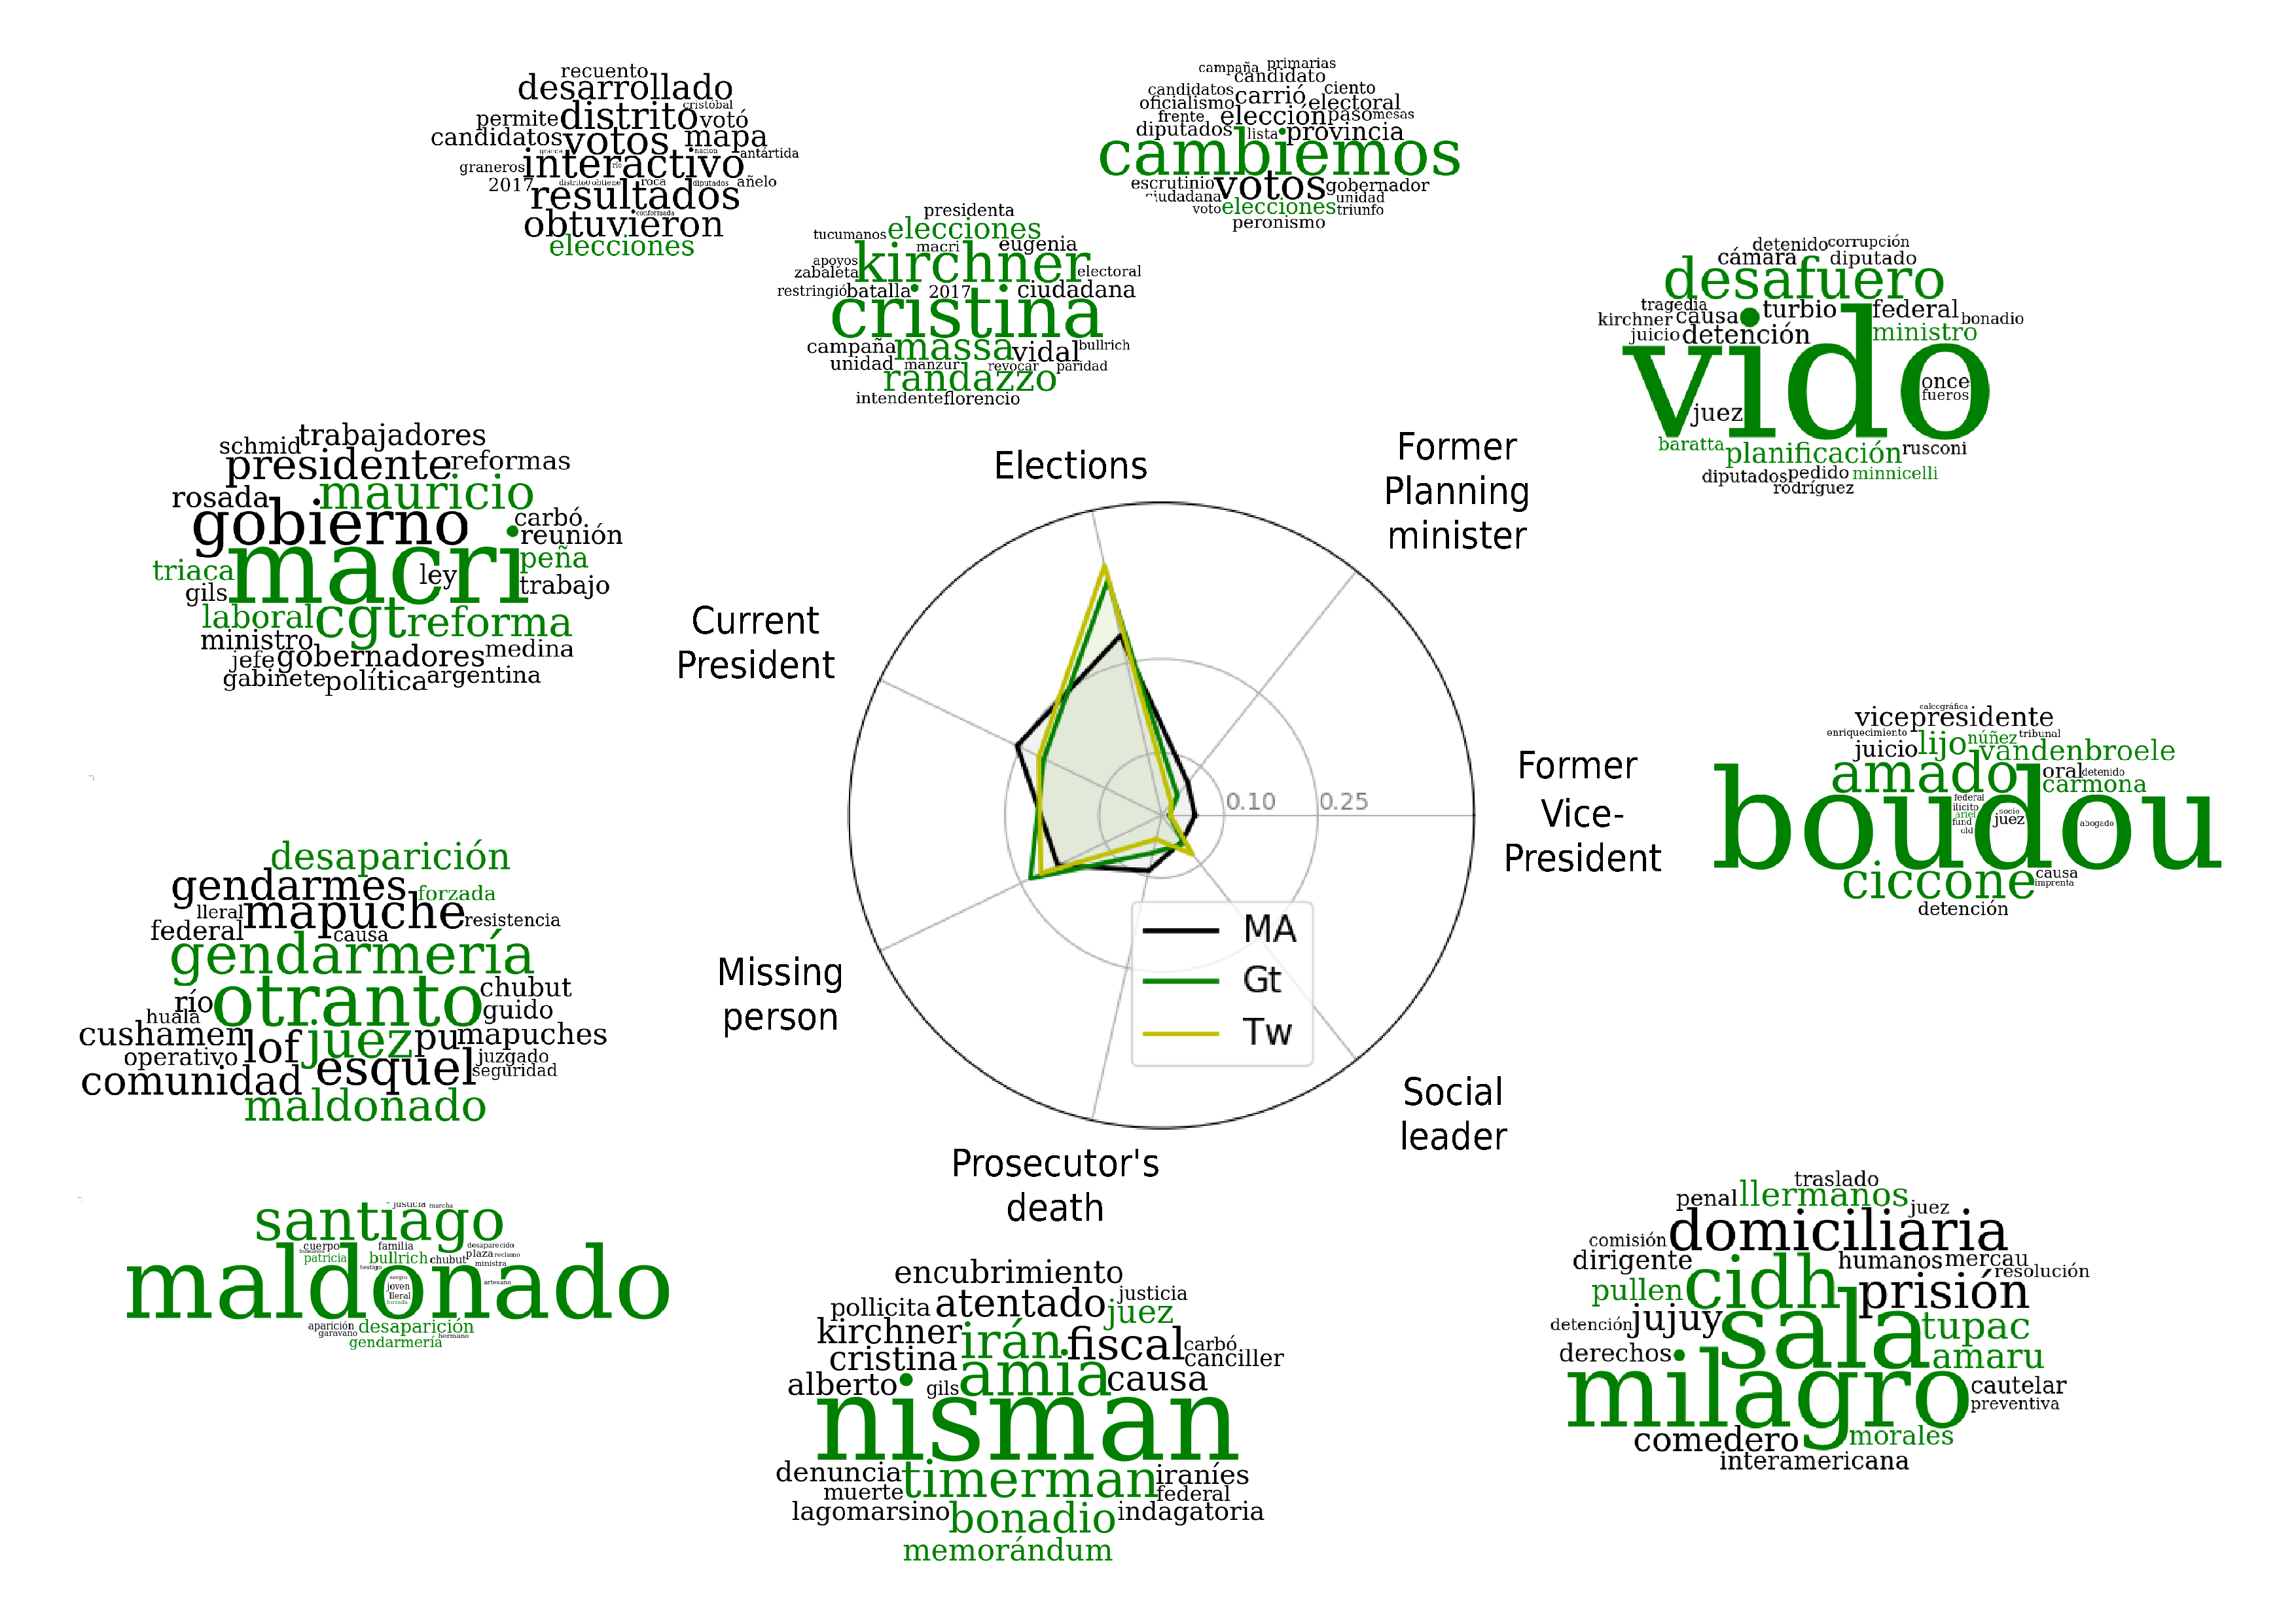
\includegraphics[width = \textwidth]{images/Fig1.pdf}
\caption{\textbf{Bump graph of the Media Agenda (MA) and Public Agenda (PA).} Topics’ names are introduced and some important events are pointed out. The curves’ width and their ordering are related to the topics’ relative weight.}
\label{fig:all_agenda}
\end{figure}
 
The topics' names are introduced in the figure, where we also point out some important events related to them.
\par In figure \ref{fig:topics_wordclouds}, we show the wordclouds of the keywords that define each topic, where the size of the word belongs to the importance in the topic's definition given by the topic detection algorithm. In green color, we point out the words involved in the Google Trends queries in order to construct the Public Agenda. The queries employed in Google Trends are specifically shown in table \ref{table:gt_all_correlation} together with the linear correlation between the topics' temporal profiles that form the Public Agenda and their counterparts in the Media Agenda.
\par In figure \ref{fig:topics_wordclouds}, we also show the radar plots of the distributions made up by averaging over time the Agendas of figure \ref{fig:all_agenda}, as a way to reduce that information which would help in farther discussions. We use radar plots as an alternative of histograms because its facility in distributions comparison.  

% Wordclouds
\begin{figure}[h]
\centering
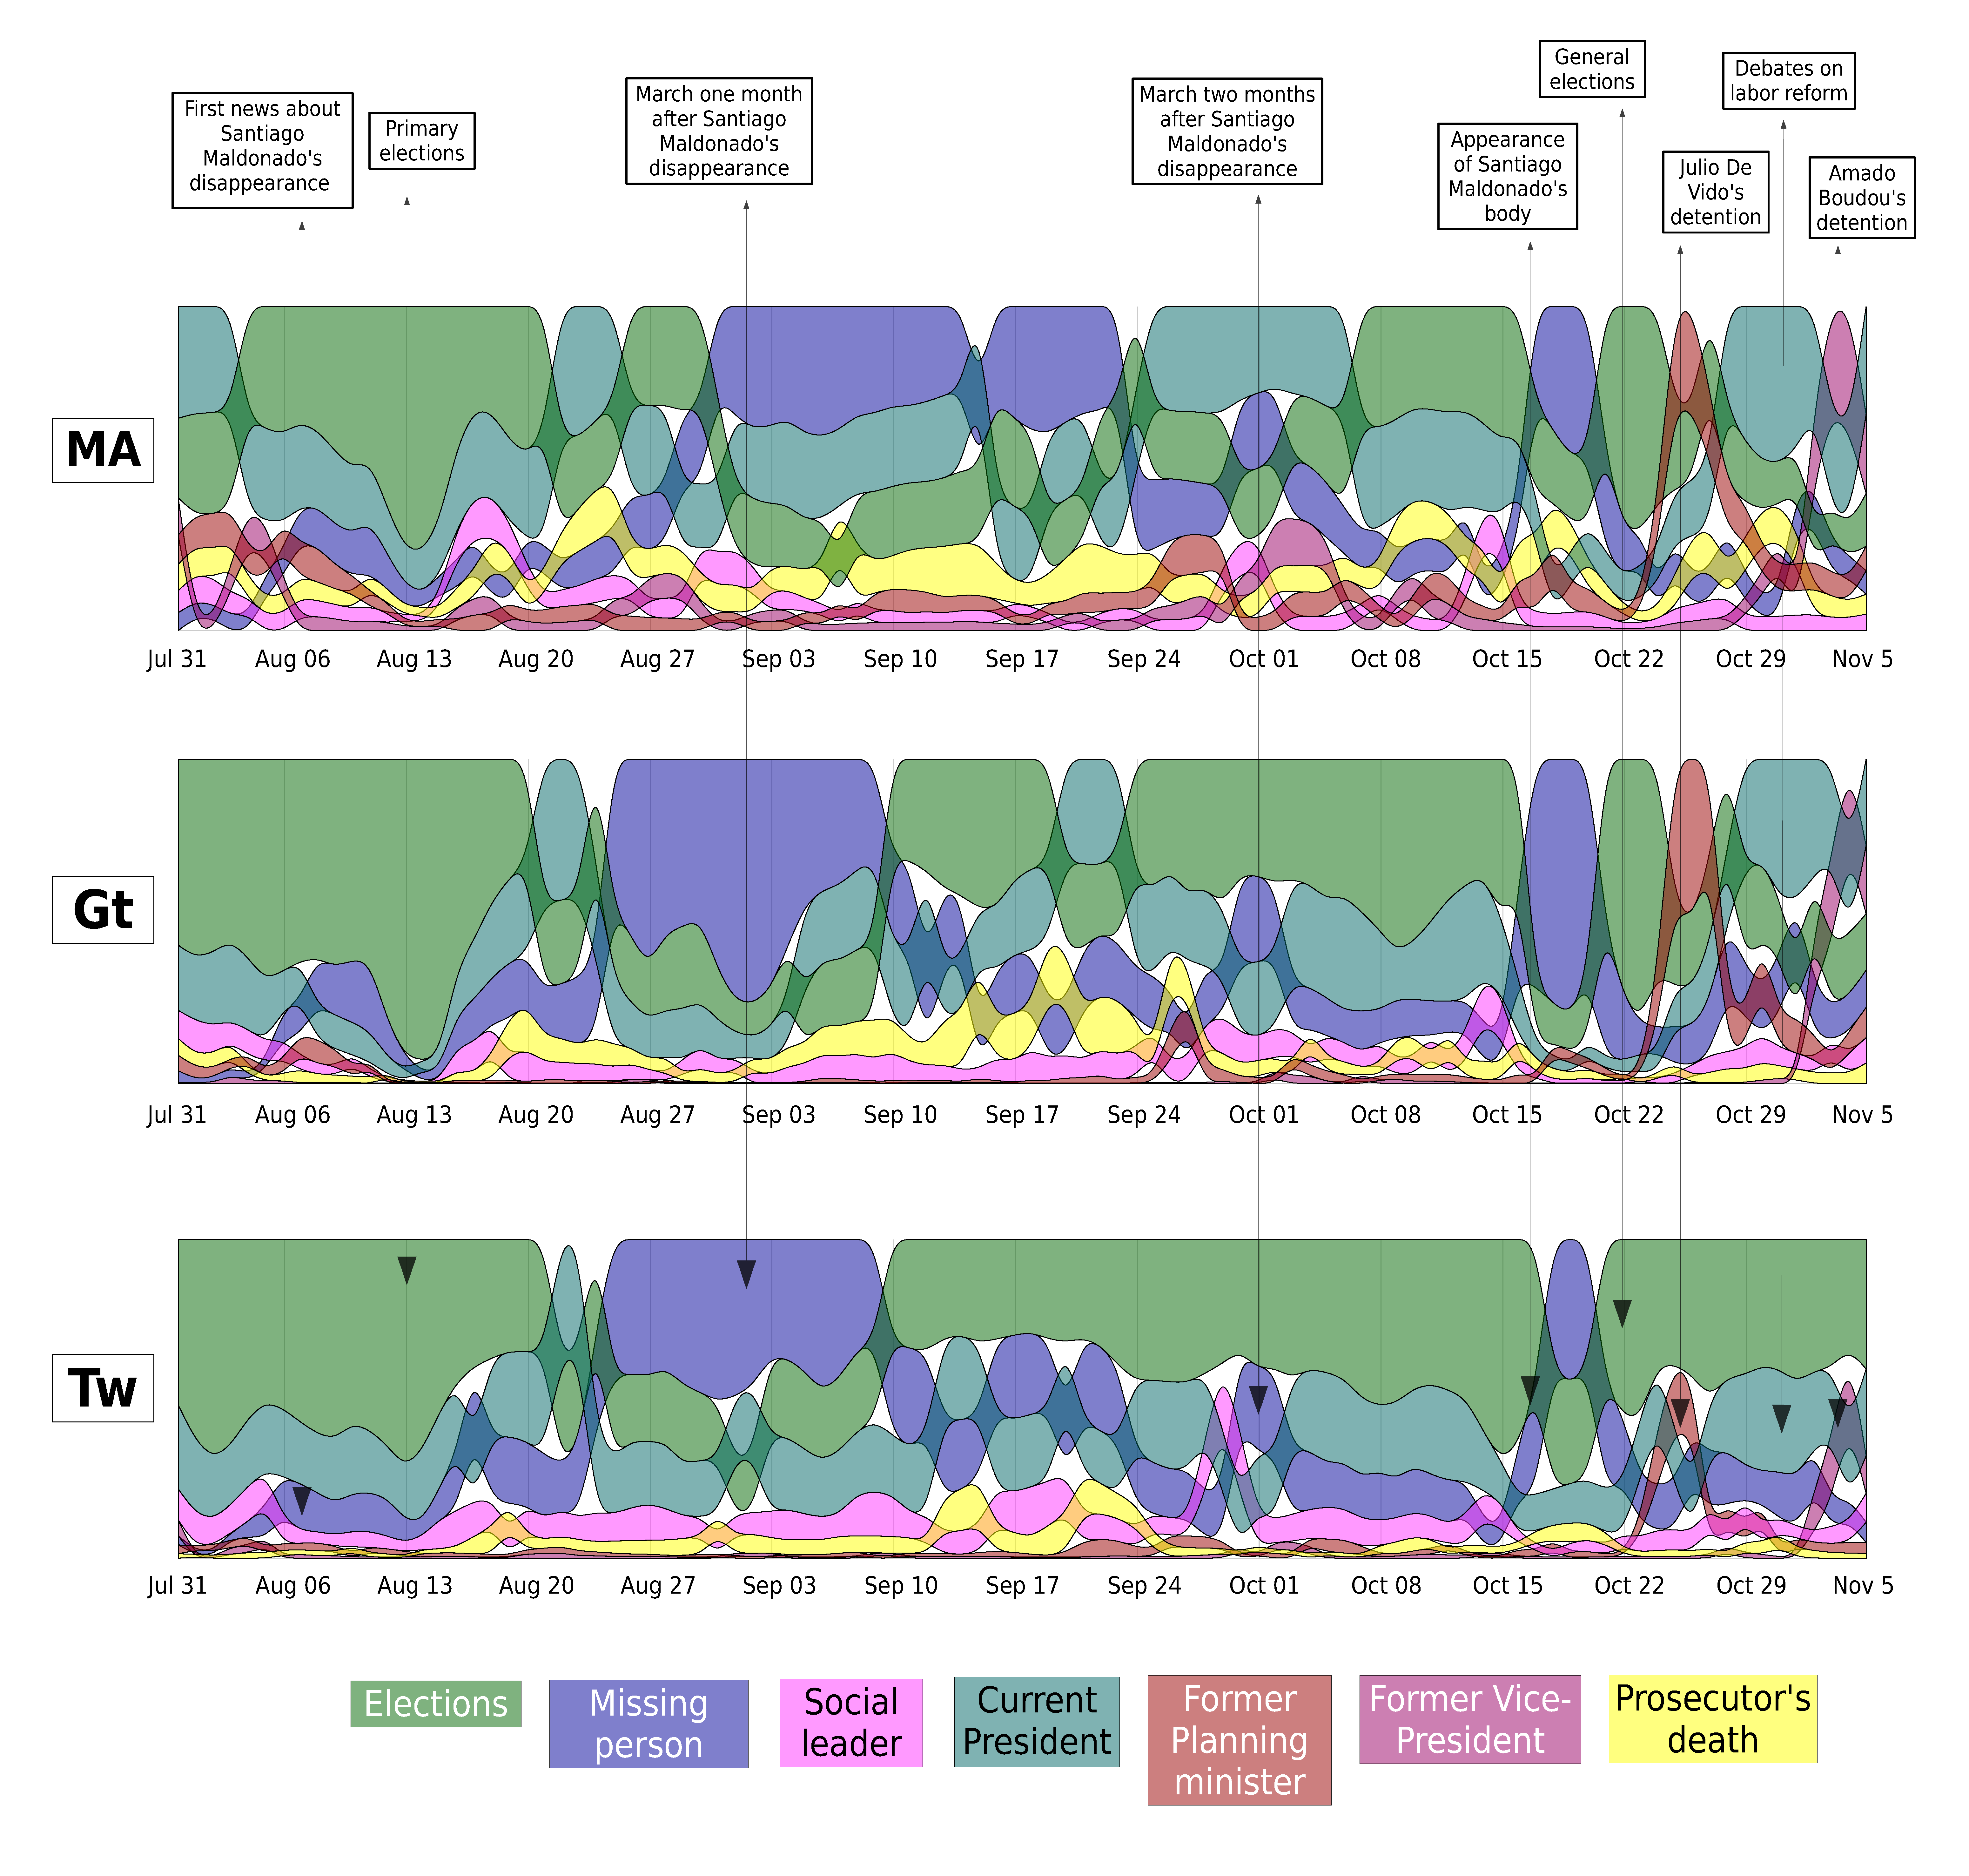
\includegraphics[width = \textwidth]{images/Fig2.pdf}
\caption{\textbf{Wordclouds and radar plot of Media and Public Agenda as an average distribution.}
In the last one, it can be seen, for instance, a greater interest of the audience in the topic Missing person than the Media. 
The wordclouds show the most important keywords involved in the definition of each topic, where in green color we show those included in the Google Trends queris (see table \ref{table:gt_all_correlation}) and therefore in our construction of the Public Agenda.
}
\label{fig:topics_wordclouds}
\end{figure}

% Table with queries and correlations
\begin{table}[h]
\centering
\resizebox{\textwidth}{!}{\begin{tabular}{llccc}
\toprule
& Google Trends query & Correlation MA and Gt & MA and Twitter & Gt and Twitter \\ 
\midrule
Elections & elecciones + cambiemos + cristina kirchner + massa + randazzo & \textbf{0.81} & \textbf{0.59} & \textbf{0.75} \\
Missing person & santiago maldonado + juez otranto + patricia bullrich + gendarmería + desaparición forzada & \textbf{0.68} & \textbf{0.76} & \textbf{0.89} \\
Former Planning minister & de vido + desafuero + ministro de planificación + minnicelli + baratta & \textbf{0.92} & \textbf{0.82} & \textbf{0.87} \\
Current President & mauricio macri + cgt + reforma laboral + peña + triaca & \textbf{0.77} & \textbf{0.75} & \textbf{0.63} \\
Social leader & milagro sala + cidh + tupac amaru + pullen llermanos + morales & \textbf{0.49} & \textbf{0.25(*)} & \textbf{0.57} \\
Prosecutor's death & nisman + amia + memorándum con irán + timerman + juez bonadio & \textbf{0.56} & \textbf{0.59} & \textbf{0.75} \\
Former Vice-President & amado boudou + ciccone + ariel lijo + vandenbroele + núñez carmona & \textbf{0.90} & \textbf{0.92} & \textbf{0.97}\\
\bottomrule
\end{tabular}}


\caption{Queries performed in Google Trends in order to made up the Public Agenda. 
We also shown the correlation between the topics' temporal profiles of the Public Agenda and their counterpart in Media Agenda.
All correlation values are statistical significant ($p < 10^{-9}$), except (*) which is significant with $p < 0.05$.}
\label{table:gt_all_correlation}
\end{table}


\par The figures introduced above show in a qualitative way the differences between the agendas, and the dynamics of the topics, i.e. the range of dates in which a given topic was an important one, for which topic it was replaced, and so on. We can see, for instance in the radar plot of figure \ref{fig:topics_wordclouds}, a more interest of the audience in the topic \emph{Missing person} than the Media, or inversely in the topic \emph{Prosecutor's death}, when we see all the period analyzed as a whole. 
\par On the other hand, the linear correlations of table \ref{table:gt_all_correlation} are in all cases positive and statistically significant, which we interpret as a form of validation of the topics found in the corpus and the keywords that describe it. 
We expected that the Media's and public's interest should generally follow a similar a pattern due to the external events, although the periods where those differ are of particular interest for us. 
A non positive (or a non significant) correlation may imply that we are not properly detecting the keywords or features that describe a particular topic, so the Google Trends' pattern would not be able to reflect a similar behavior that its counterpart in the Media.

% Temporal_profiles
\begin{figure}[h]
\centering
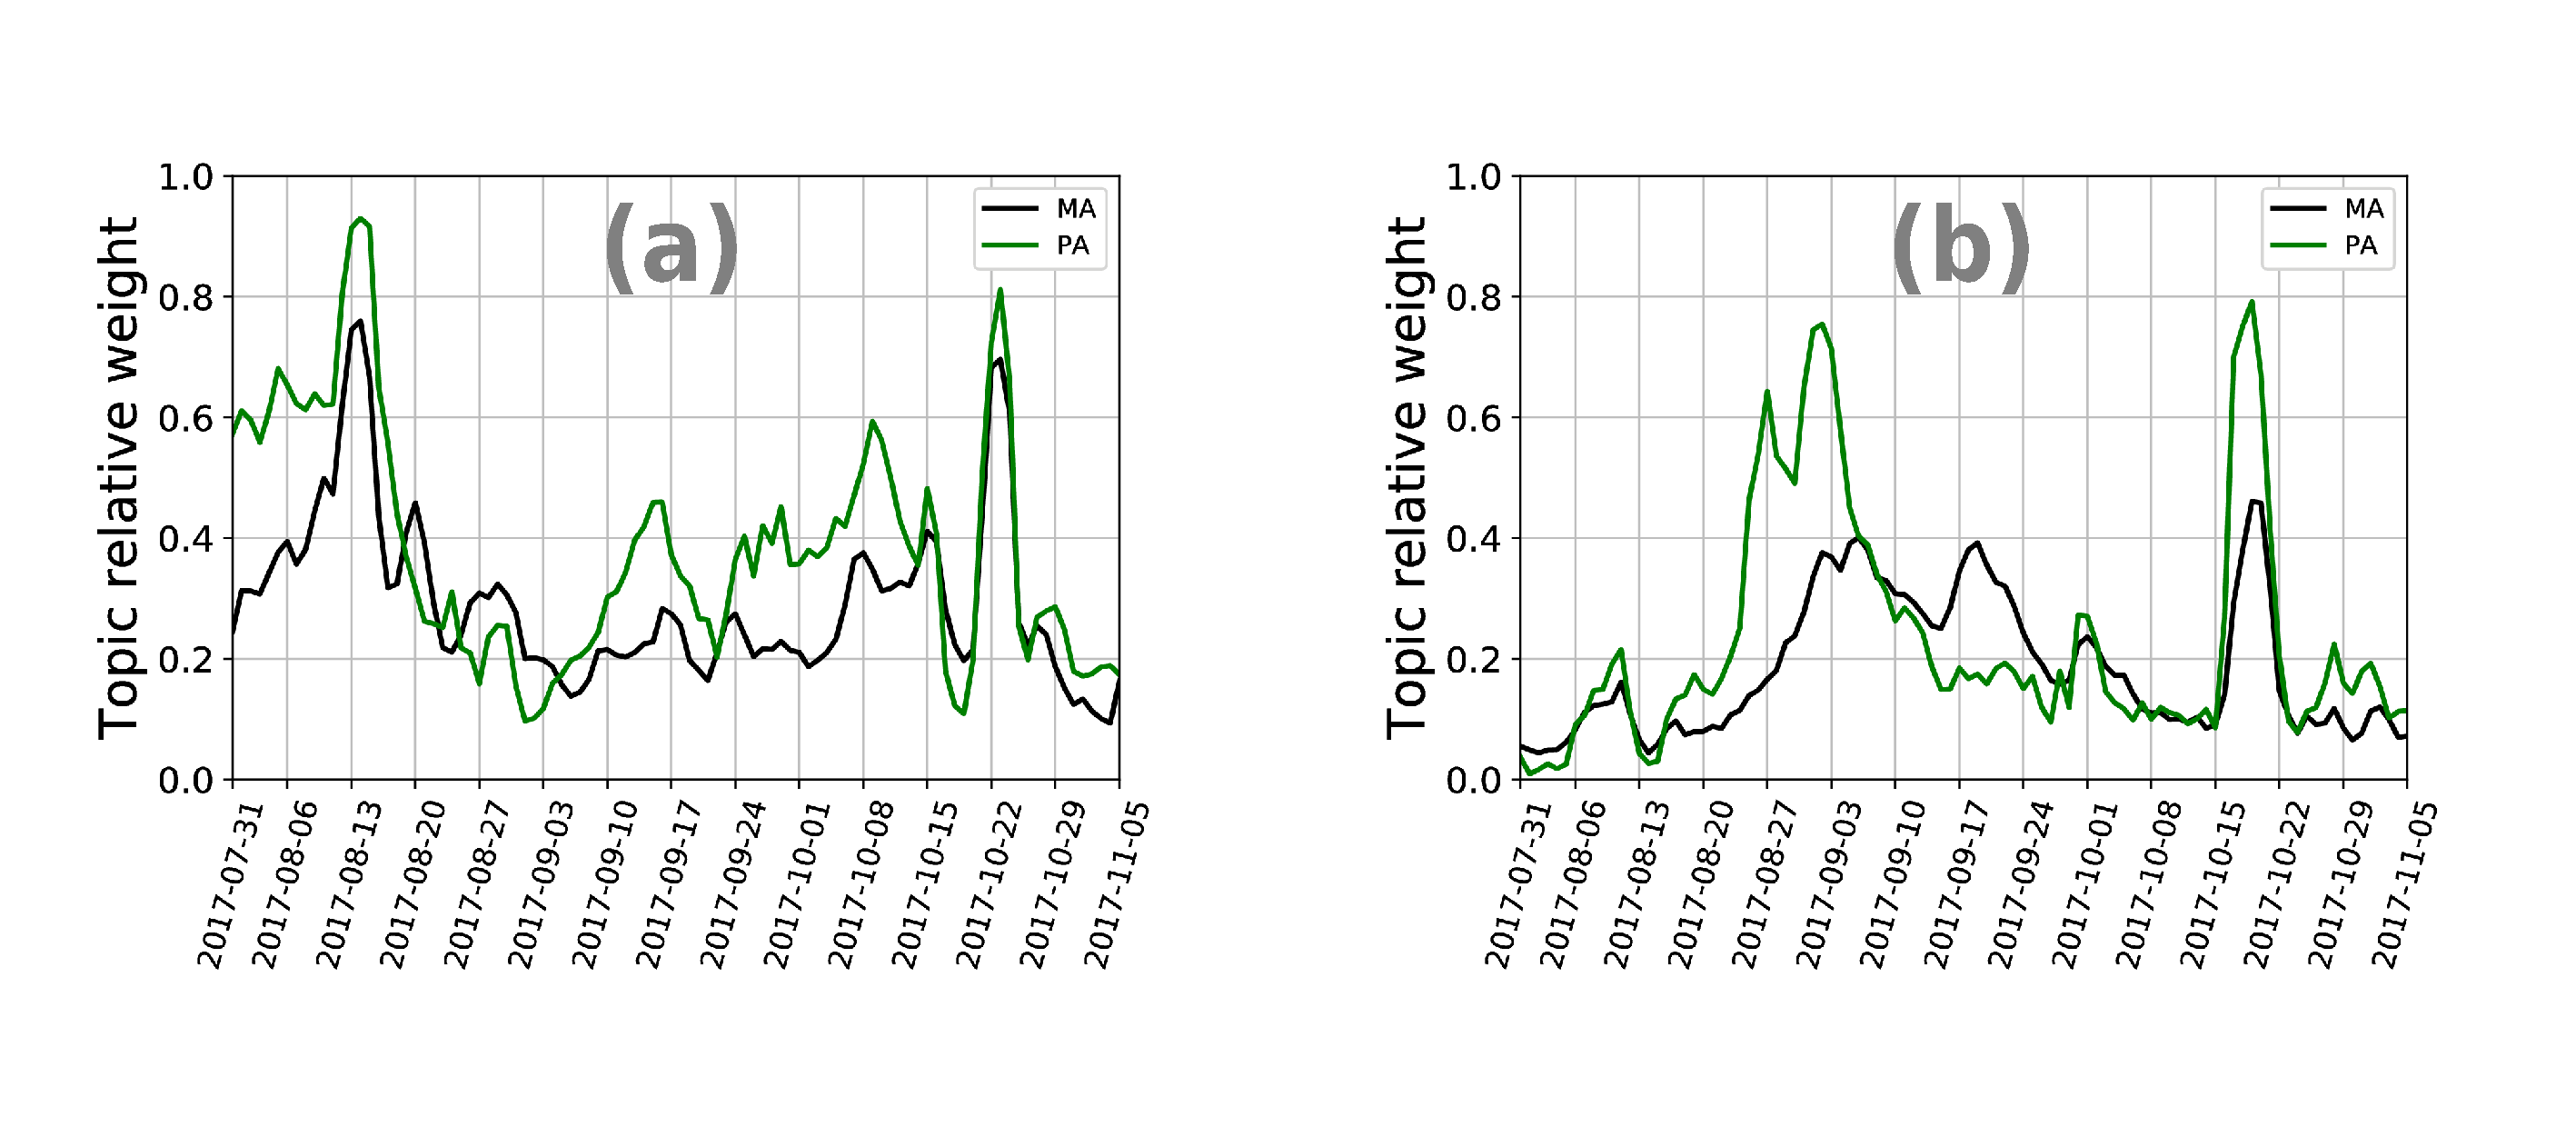
\includegraphics[width = \textwidth]{images/Fig2_5.pdf}
\caption{\textbf{AUXILIAR IMAGE: Temporal profiles.}
Elections (left) and Missing Person (right).
}
\end{figure}

\subsection{A quantitative approach}

\subsubsection{Agenda diversity}

% Agenda diversity

\par In order to quantify the similarities and differences between the Media Agenda and the Public Agenda, we start by asking how is the distribution of each agenda among the topic's space. In particular, we measure how diverse is each agenda. Following \cite{boydstun2014importance}, we calculate the normalized Shannon's entropy ($H$, see eq.\ref{eq:shannon_entropy}) in order to measure the diversity of the \textbf{MA} and \textbf{PA}.
\par In figure \ref{fig:shannon_entropy_agendas} we can see the value of $H$ as a function of time. We can see that there are periods where the diversity is lower than the usual. In particular, we pay attention to four dates in the Public Agenda which we detect as outliers of the typical behavior. The small value in the diversity is due to the fact that the most important topic attracts practically all the attention of the public, as can be seen in the radar plots included also in figure \ref{fig:shannon_entropy_agendas}. 
Two of the points belong to the topic \emph{Elections} and coincide with the primary and general legislative elections that took place in August 13th and October 22th. In the other hand, the other two point belong to the topic \emph{Missing person}: The first one a month after the disappearance of Santiago Maldonado, and the second one, when the Santiago Maldonado's body was found, a few days before the general legislative election (see section \ref{sec:Context}).

\begin{figure}[h]
\centering
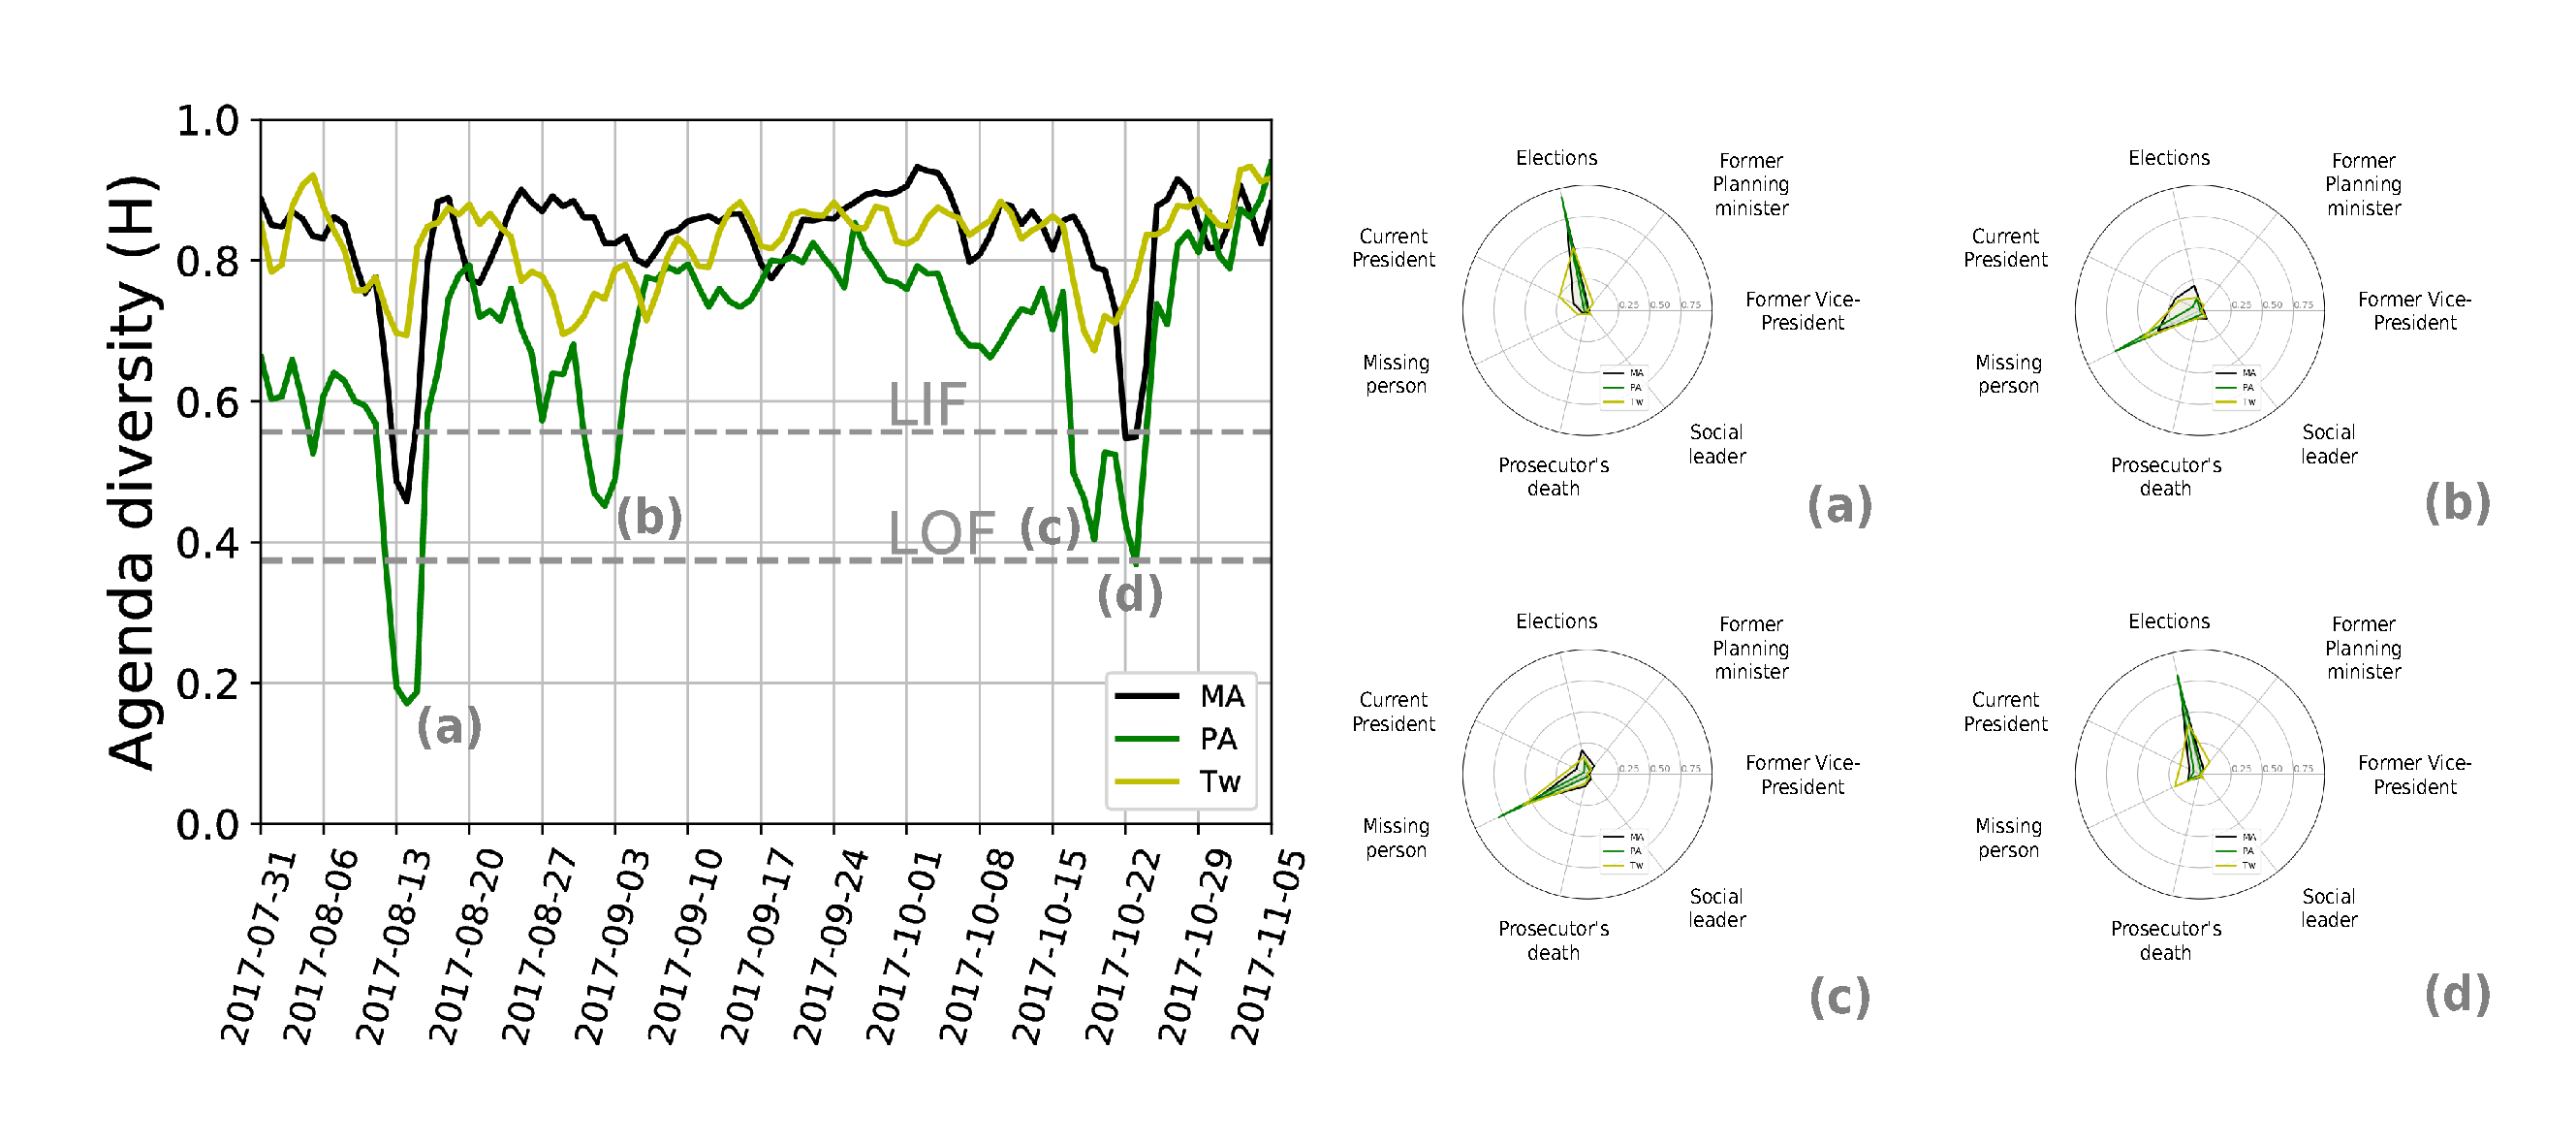
\includegraphics[width = \textwidth]{images/Fig3.pdf}
\caption{\textbf{Shannon entropy (H) as a measure of agenda diversity.} The Public Agenda show a less diverse behavior than the Media Agenda as can be seen in the left figure. The lower fences are shown in order to identify outliers. The related radar plots shows that those dates when the agenda has a low diversity, the most important topic catches the most public’s attention}
\label{fig:shannon_entropy_agendas}
\end{figure}

\par From the measure of $H$ we can also see that the median of the Public Agenda diversity ($H_{PA} = 0.70$) is lower than the each the Media Agenda's one ($H_{MA} = 0.85$) being this difference statistical significant ($p < 10^{-9}$).
We conclude that its an important fact about audience behavior: given a finite set of topics, \textbf{the Public Agenda is less diverse than the Media Agenda}, because the public seems to focus more in the most important topic than the Media can do.

\subsubsection{Public Agenda's distance}

% Jensen-Shannon distance between PA and MA

\par The measurement of the Shannon's entropy made above is an independent property of each distribution. 
Here we directly compare the Agendas by computing the Jensen-Shannon distance. We again identify outliers and aim to interpret them.
In figure \ref{fig:jensen_shannon_gt} we show the Jensen-Shannon distance as a function of time. We inspect three points that seems to be of particular interest. In all cases, the radar plots shows that a greater distance is associated with a more interest of public in the topic \emph{Missing person}. 
\par Points \textbf{(b)} and \textbf{(c)} shows that both the public and the Media are interest in that topic, but the Media have to cover other topics, so the distance value can be seen as a derivation of the diversity effect discussed in the last section.
However point \textbf{(a)} seems to show an interest of the public in the topic \emph{Missing person} that it is not reflected in the Media. In figure \ref{fig:all_agenda} we can see that this topic reached the first place in public's interest before that in the Media. We associate this fact with a campaign made in social media like Facebook and Twitter in August 26th, that paid for the appearance of Santiago Maldonado and had a great repercussion, maybe at first underestimated by the Media (see section \ref{sec:Context}). 
\par It is important to recall that it is our interpretation based on the knowledge of the context, and that we are not studying causality, i.e. we can't say, for instance, that in this case the Public Agenda set the Media Agenda. However, the Jensen-Shannon distance, in conjunction with the measurement of the agenda diversity given by the Shannon entropy, give an insight of independent behavior of the Public and the Media, and its identification can be a starting point to study the Media reaction to a change in audience's interests.
 
\begin{figure}[h]
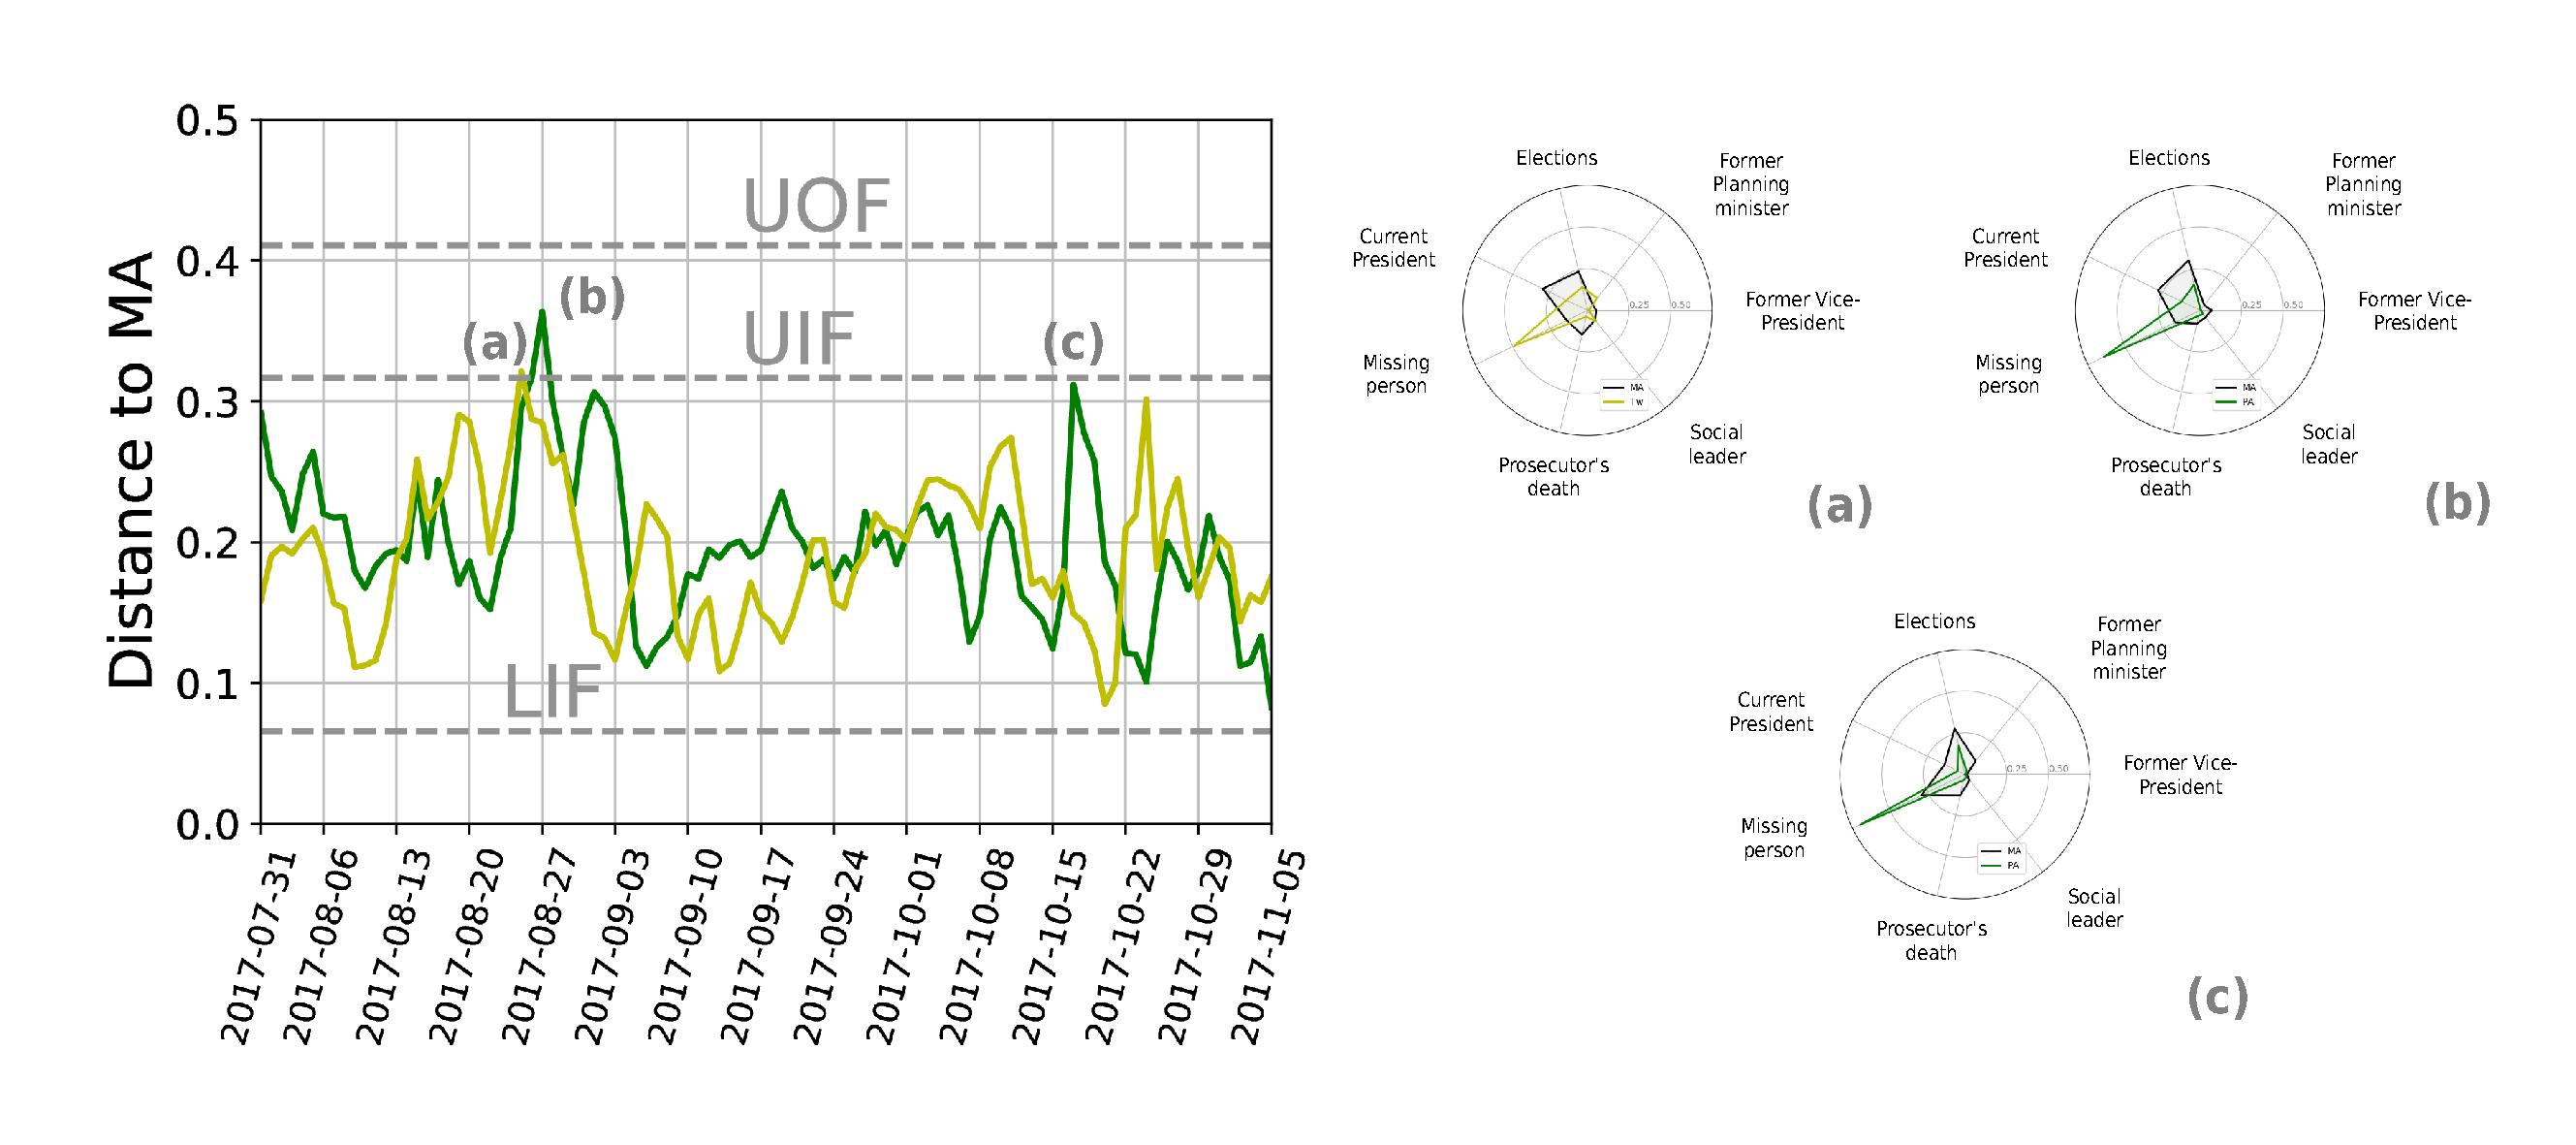
\includegraphics[width = \textwidth]{images/Fig4.pdf}
\caption{\textbf{Jensen Shannon distance between the Media Agenda and the Public Agenda as a function of time} (with the fences pointed out). The larger distances are due to a greater interest of the audience in the topic \emph{Missing person} which leads to lesser interest in the other topics, which the Media has to cover, maybe except in the date (a) where the Media seems not to anticipate the public interest in the mentioned topic.}
\label{fig:jensen_shannon_gt}
\end{figure}


\subsection{Media Agenda: differences between newspapers}

\par In this section we leave aside the Public Agenda and we study how the Media agenda varies when one consider the newspapers separately. 
In figure \ref{fig:news_agenda} we show the bump charts which belongs to each newspaper analogously to figure \ref{fig:all_agenda}.
The topics are the same introduced in the wordclouds of figure \ref{fig:topics_wordclouds}, but at computing the topics' weights the articles are separated by newspaper. 
We also show the radar plots showing the average distribution, as made in figure \ref{fig:topics_wordclouds}. 
\par In figure \ref{fig:news_agenda} we can see in a qualitative way the slightly differences between the newspapers' agendas.
For instance, we can see how \emph{Página 12} gave more importance to the topics \emph{Missing person} and \emph{Social leader}, while it did not pay too much attention to the \emph{Former Planning minister} as the others did.

% Jensen shannon distance of Dynamic way
\begin{figure}[h]
\centering
\includegraphics[width = \textwidth]{images/Fig5.pdf}
\caption{\textbf{Bump charts of newspapers' Agenda and radar plot of the average distributions.} The figure shows, in a qualitative way, the differences between the mentioned agendas, for instance, the greater interest of Página 12 (P12) in the \emph{Missing person}’s topic and its slightly lesser interest in the \emph{Former Planning minister} respect to the other newspapers.}
\label{fig:news_agenda}
\end{figure}

\subsubsection{Independent behavior}

\par In other to detect an independent behavior of a newspaper respect the others we again calculate the Jensen-Shannon distance between the newspapers agenda and the Media Agenda.
Note that this is the distance between the distributions of figure \ref{fig:news_agenda} and the top panel of figure \ref{fig:all_agenda}.
\par In figure \ref{fig:jensen_shannon_news} we show the Jensen-Shannon distance is a function of time.
We detect three points as outliers, although we discard the point \textbf{(b)} due to the low information of \emph{Infobae} in that period. 
The other two points belongs to a difference between \emph{Página 12} and the other newspapers. 
We interpret that the coverage of the topic \emph{Missing person} is the principal cause of the outliers.
\emph{Página 12} paid more attention to it than the Media Agenda at point \textbf{(a)} when the first notices of the Santiago Maldonado's disappearance before the primary elections, and in point \textbf{(c)} when a march two months after the disappearance took place, and had not the same coverage as the other march a month before (see section \ref{sec:Context}). Also, in point \textbf{(c)}, it can be seen a greater coverage of \emph{Página 12} in the topic \emph{Social leader} while the others seemed to be more interested in the topic \emph{Former Vice-President}.

% Jensen shannon distance of Dynamic way
\begin{figure}[h]
\centering
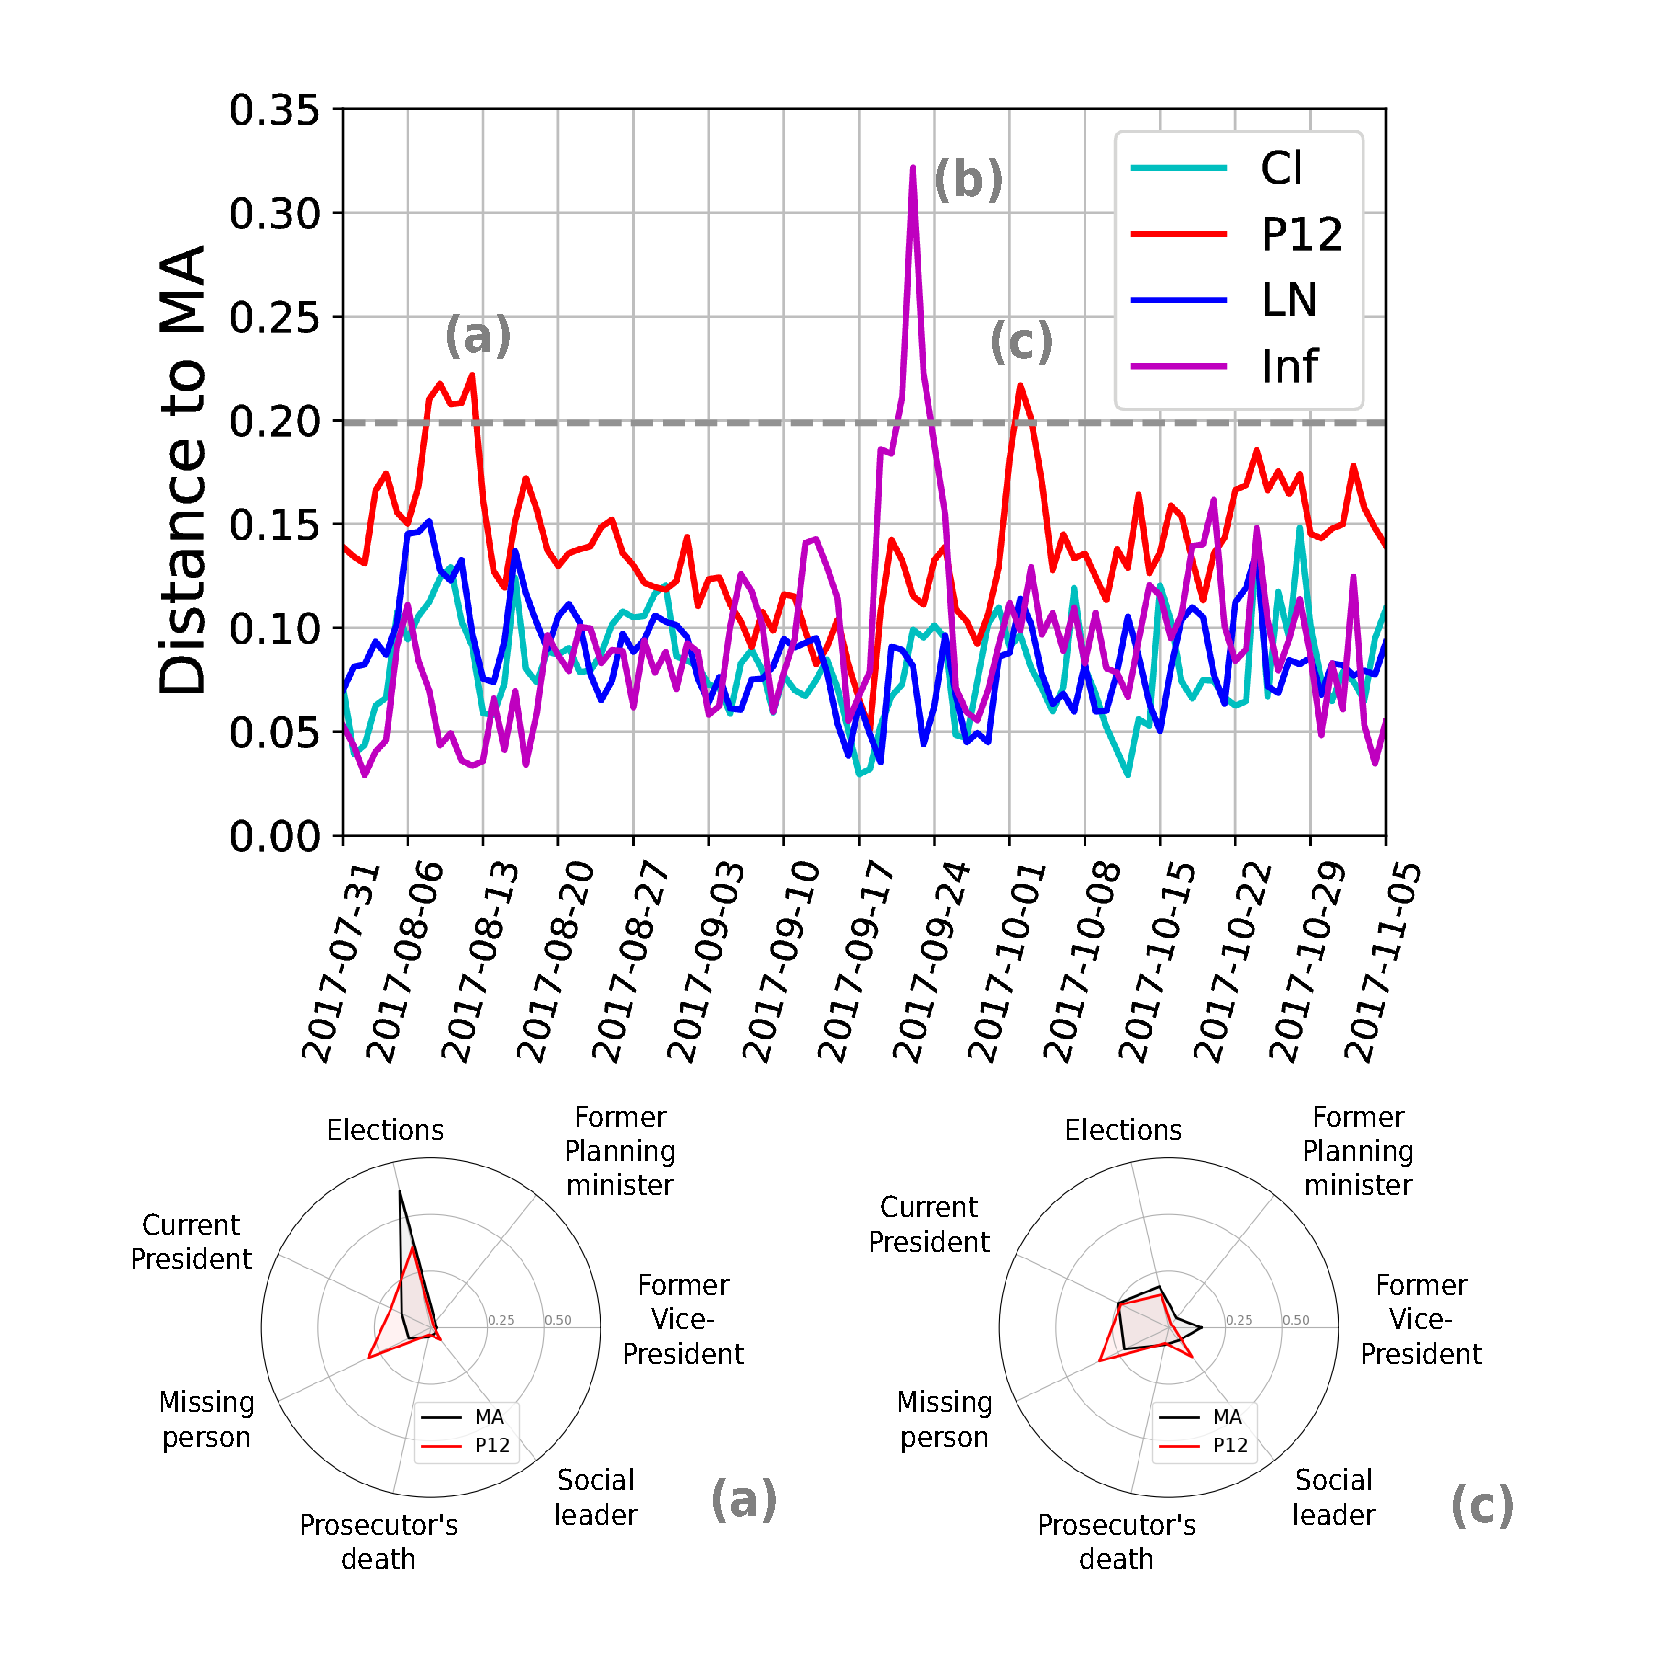
\includegraphics[width = \textwidth]{images/Fig6.pdf}
\caption{\textbf{Jensen Shannon distance between the newspapers’ agenda and the Media Agenda as a function of time.} \emph{Página 12} (P12) shows the more different behavior, motivated again by its interest in the \emph{Missing person} and \emph{Social leader} topics as can be seen in the radar plots which belongs to points (a) and (c). 
The anomalous behavior of \emph{Infobae} (Inf) at point (b) is due to few articles around that date in our database, therefore we ignore its radar plot.}
\label{fig:jensen_shannon_news}
\end{figure}

\subsubsection{Coverage bias}

\par The greater coverage in the topic \emph{Missing person} by \emph{Página 12} is even more clear if we inspect the temporal profile of the topic and compare the coverage given by each newspaper. A difference in the coverage is what it is called \emph{coverage bias}.
In figure \ref{fig:topics_temporal_profiles} we show the temporal profile of the topic \emph{Missing person} (panel (a)) and the topic \emph{Former Planning minister} in panel (b), as an example where the behavior is the opposite, as can be seen below.

\begin{figure}[h]
\centering
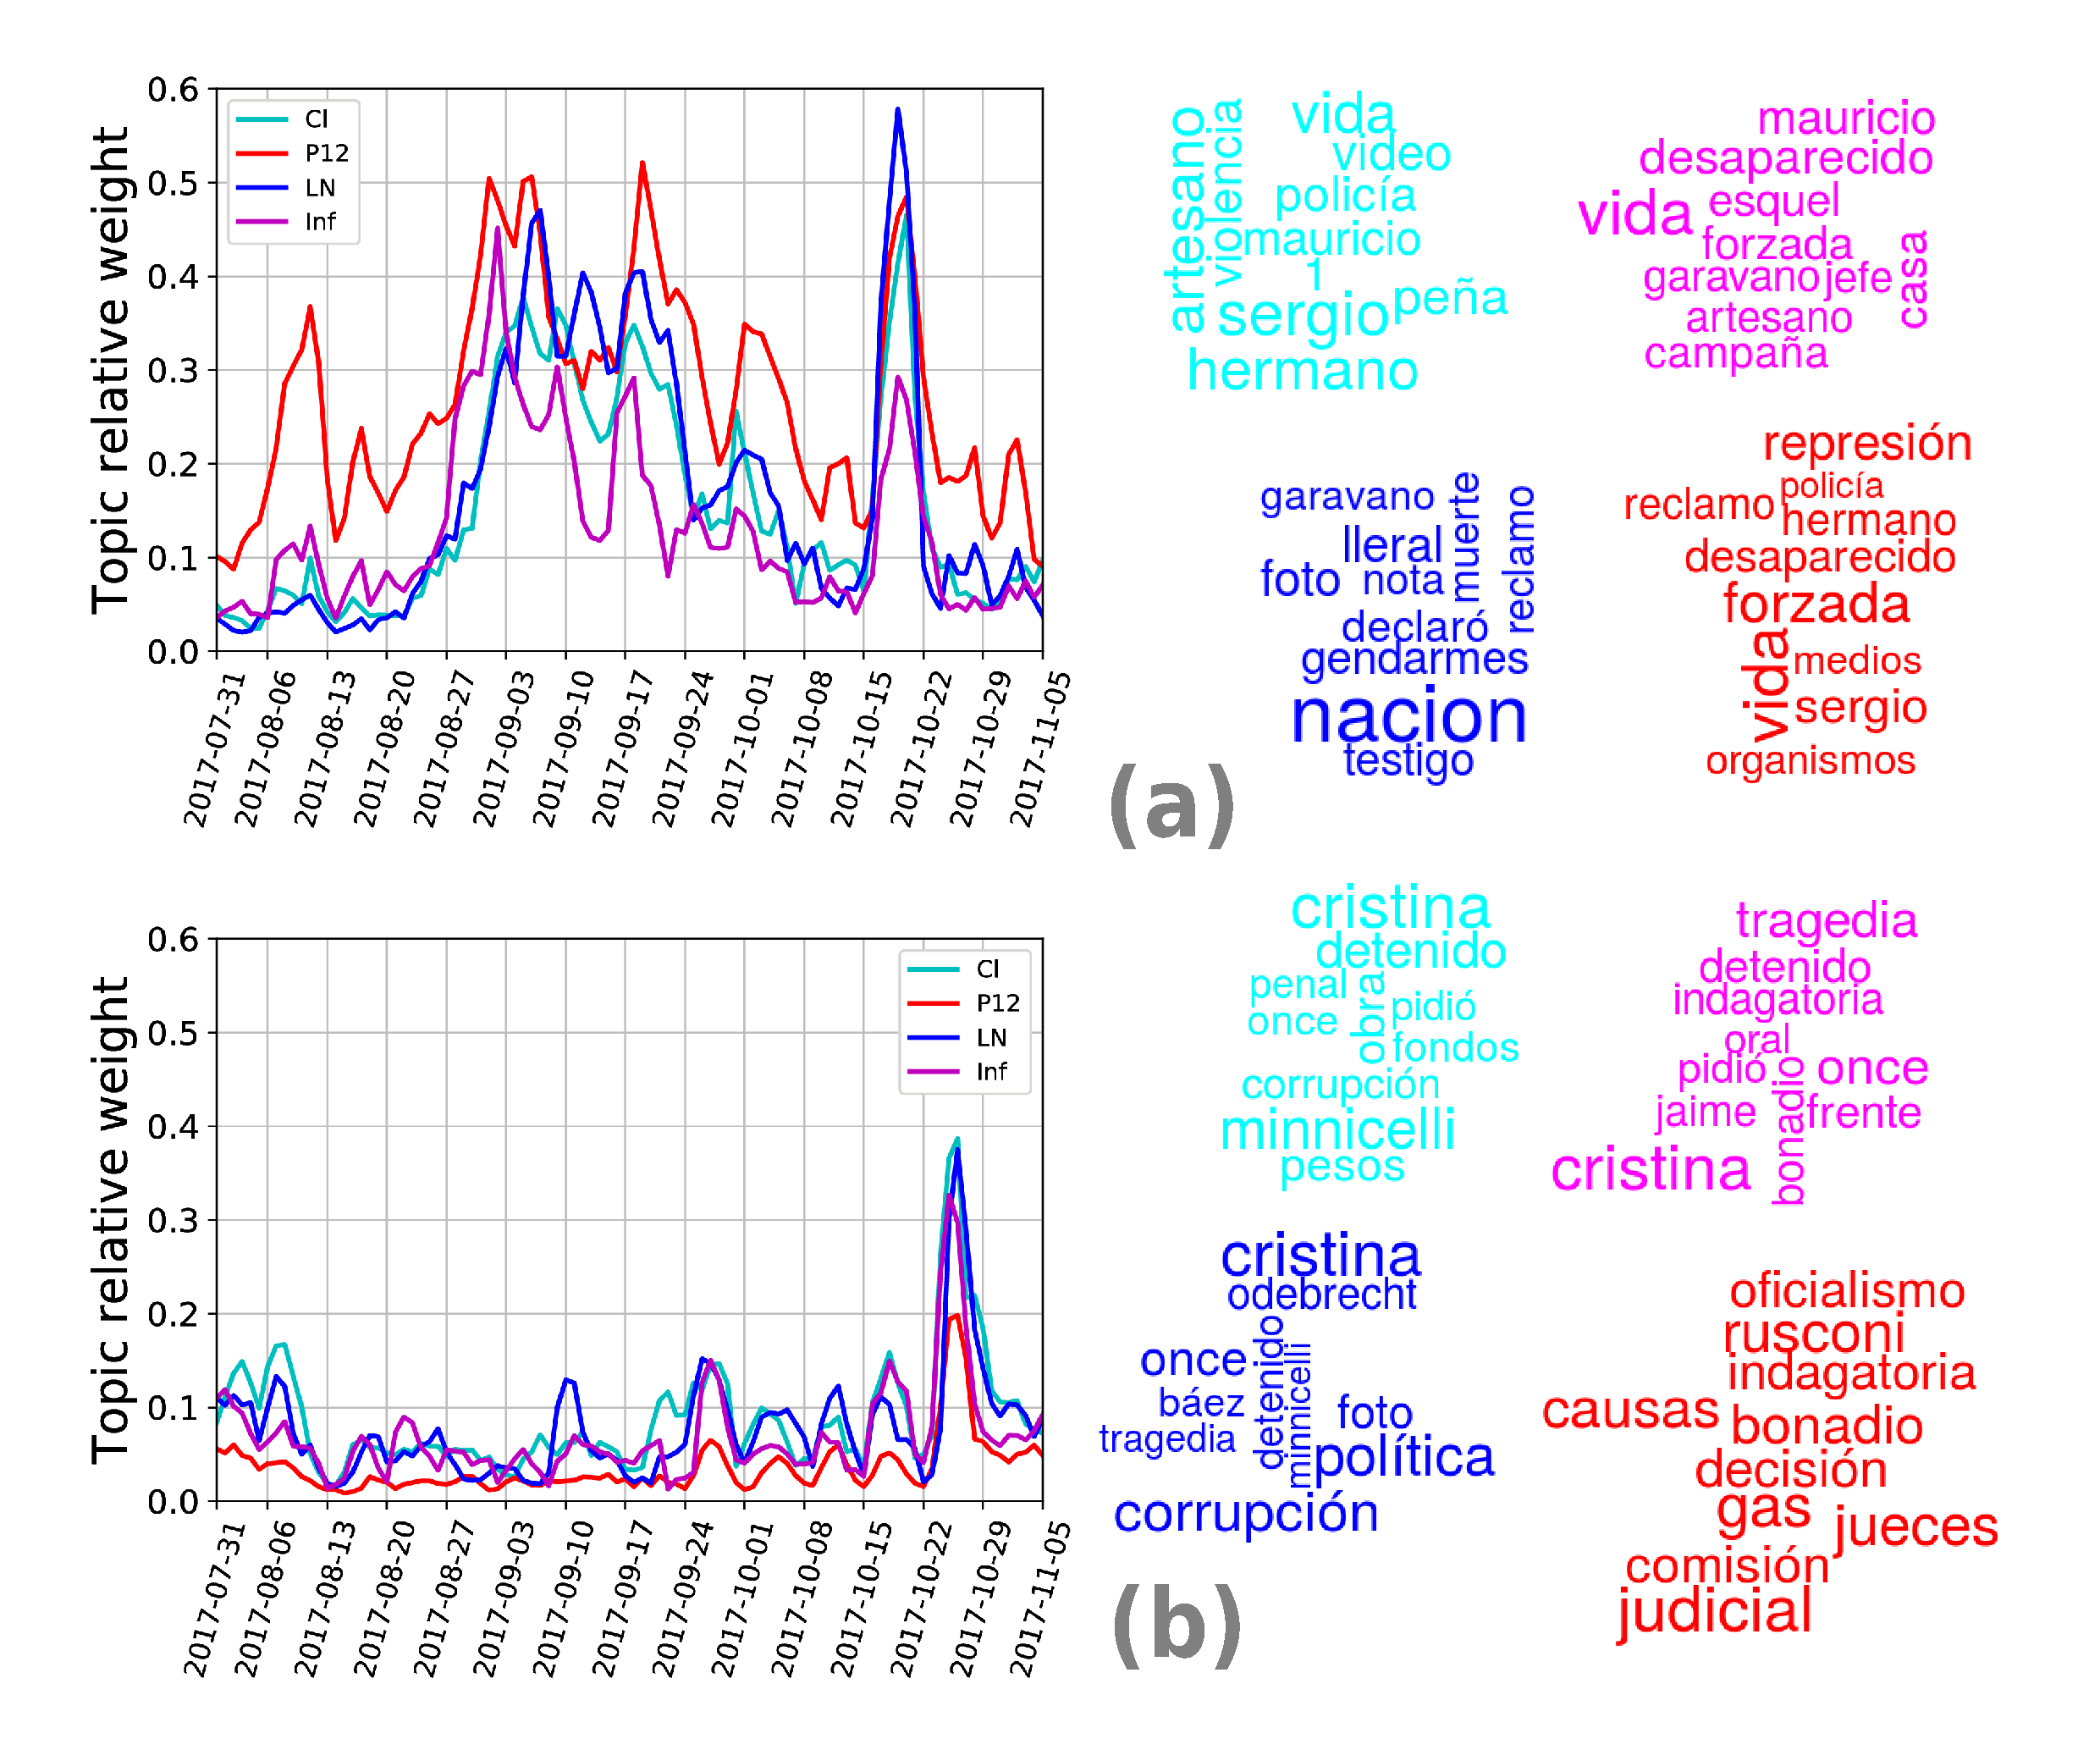
\includegraphics[width = \textwidth]{images/Fig7.pdf}
\caption{\textbf{Relative weight of the topics (a) \emph{Missing person}, and (b) \emph{Former Planning Minister}, and wordclouds of frequent newspapers' keywords}. We interpreted the differences shown in certain periods as an indicator of coverage bias. For instance, in figure (a) Página 12 pays a greater attention in the first days. In the wordclouds, we show which of the defining words are more frequently used by the corresponding newspaper. Most of them are less informative, but other seems to represent a first approximation in the study of framing.}
\label{fig:topics_temporal_profiles}
\end{figure}

\par From panel (a) of figure \ref{fig:topics_temporal_profiles}, we can see a more coverage of \emph{Página 12} respect the other newspapers at the first of the period. We can for instance quantify this difference by the median of the signals. If we focus in the period between July 31th and August 27th, the median of the topic relative weight for \emph{Página 12} is roughly 0.14 and this is statistically significant larger ($p < 10^{-7}$) than other medians, which are lower than 0.05.
Analyzing the same period, but in panel (b), we again can show that the median in \emph{Página 12}, which is roughly 0.01, is lower than the others, which oscillate around 0.05 ($p<10^{-3}$)
This quantification is proposed as method of studying coverage bias in the context of the methodology implemented in our work. 

\par Finally, in figure \ref{fig:topics_temporal_profiles} we also show wordclouds of topic's keywords but separate those that are most frequent mentioned by each newspaper, filtering the words that are common to all and basically define the factual details of the topic.
Although most words are less informative, some are interesting to inspect, for instance, the word \emph{represión} (repression) when \emph{Pagina 12} talks about the topic \emph{Missing Person} and the word \emph{Cristina} (Fernández de Kirchner) which is employed by all newspapers except \emph{Pagina 12} when talk about the topic \emph{Former Planning minister} (see section \ref{sec:Context}).
We don't go farther but we think that a more deeply study of topics' keywords is a first approximation in the study of framing, which will constitute the core of futures works.


\section{Conclusions}

\par The study of Mass Media, and in particular the agenda setting theory, can be empowered by the used of data mining or machine learning algorithms. 
In this work, through the implementation of a topic detection algorithm we could describe the Agenda of the Media as a distribution which evolves over time and which is defined in a topic's space which emerges from the analysis of the corpus.
This gave us an insight of how we can construct and follow the Public's interests, the Public Agenda, in order to compare with the Media Agenda, i.e. Media interests. 
\par Given the Agendas, we found that the Public one is usually less diverse than the Media, showing that when there is a very attractive topic, the audience focus on this one, when the Media has to cover the other too. 
On the other hand, the measurement of distances between Agendas can be employed to rapidly detect periods when the Public may have an independent behavior respect to the Media. The methodology implemented here also allow us to detect coverage bias in newspapers and gave us a first approximation in the theory of framing. 
\par We hope that some of the elements studied here will give us insights at the time of proposing a mathematical model about Mass Media and Public interaction. Future works may include a more systematic study and its extension to international Media, a deeper study of framing through topic detection and sentiment analysis, and a more quantitave analysis about causation.


\section*{Content}
Text and results for this section, as per the individual journal's instructions for authors. %\cite{koon,oreg,khar,zvai,xjon,schn,pond,smith,marg,hunn,advi,koha,mouse}

\section*{Section title}
Text for this section \ldots
\subsection*{Sub-heading for section}
Text for this sub-heading \ldots
\subsubsection*{Sub-sub heading for section}
Text for this sub-sub-heading \ldots
\paragraph*{Sub-sub-sub heading for section}
Text for this sub-sub-sub-heading \ldots
In this section we examine the growth rate of the mean of $Z_0$, $Z_1$ and $Z_2$. In
addition, we examine a common modeling assumption and note the
importance of considering the tails of the extinction time $T_x$ in
studies of escape dynamics.
We will first consider the expected resistant population at $vT_x$ for
some $v>0$, (and temporarily assume $\alpha=0$)
%
\[
 E \bigl[Z_1(vT_x) \bigr]= E
\biggl[\mu T_x\int_0^{v\wedge
1}Z_0(uT_x)
\exp \bigl(\lambda_1T_x(v-u) \bigr)\,du \biggr].
\]
%
If we assume that sensitive cells follow a deterministic decay
$Z_0(t)=xe^{\lambda_0 t}$ and approximate their extinction time as
$T_x\approx-\frac{1}{\lambda_0}\log x$, then we can heuristically
estimate the expected value as
%
\begin{eqnarray}\label{eqexpmuts}
E\bigl[Z_1(vT_x)\bigr] &=& \frac{\mu}{r}\log x
\int_0^{v\wedge1}x^{1-u}x^{({\lambda_1}/{r})(v-u)}\,du
\nonumber\\
&=& \frac{\mu}{r}x^{1-{\lambda_1}/{\lambda_0}v}\log x\int_0^{v\wedge
1}x^{-u(1+{\lambda_1}/{r})}\,du
\nonumber\\
&=& \frac{\mu}{\lambda_1-\lambda_0}x^{1+{\lambda_1}/{r}v} \biggl(1-\exp \biggl[-(v\wedge1) \biggl(1+
\frac{\lambda_1}{r}\biggr)\log x \biggr] \biggr).
\end{eqnarray}
%
Thus we observe that this expected value is finite for all $v>0$ (also see \cite{koon,khar,zvai,xjon,marg}).
%\nocite{oreg,schn,pond,smith,marg,hunn,advi,koha,mouse}

%%%%%%%%%%%%%%%%%%%%%%%%%%%%%%%%%%%%%%%%%%%%%%
%%                                          %%
%% Backmatter begins here                   %%
%%                                          %%
%%%%%%%%%%%%%%%%%%%%%%%%%%%%%%%%%%%%%%%%%%%%%%

\begin{backmatter}

\section*{Competing interests}
  The authors declare that they have no competing interests.

\section*{Author's contributions}
    Text for this section \ldots

\section*{Acknowledgements}
  Text for this section \ldots
%%%%%%%%%%%%%%%%%%%%%%%%%%%%%%%%%%%%%%%%%%%%%%%%%%%%%%%%%%%%%
%%                  The Bibliography                       %%
%%                                                         %%
%%  Bmc_mathpys.bst  will be used to                       %%
%%  create a .BBL file for submission.                     %%
%%  After submission of the .TEX file,                     %%
%%  you will be prompted to submit your .BBL file.         %%
%%                                                         %%
%%                                                         %%
%%  Note that the displayed Bibliography will not          %%
%%  necessarily be rendered by Latex exactly as specified  %%
%%  in the online Instructions for Authors.                %%
%%                                                         %%
%%%%%%%%%%%%%%%%%%%%%%%%%%%%%%%%%%%%%%%%%%%%%%%%%%%%%%%%%%%%%

% if your bibliography is in bibtex format, use those commands:
\bibliographystyle{bmc-mathphys} % Style BST file (bmc-mathphys, vancouver, spbasic).
\bibliography{bmc_article}      % Bibliography file (usually '*.bib' )
% for author-year bibliography (bmc-mathphys or spbasic)
% a) write to bib file (bmc-mathphys only)
% @settings{label, options="nameyear"}
% b) uncomment next line
%\nocite{label}

% or include bibliography directly:
% \begin{thebibliography}
% \bibitem{b1}
% \end{thebibliography}

%%%%%%%%%%%%%%%%%%%%%%%%%%%%%%%%%%%
%%                               %%
%% Figures                       %%
%%                               %%
%% NB: this is for captions and  %%
%% Titles. All graphics must be  %%
%% submitted separately and NOT  %%
%% included in the Tex document  %%
%%                               %%
%%%%%%%%%%%%%%%%%%%%%%%%%%%%%%%%%%%

%%
%% Do not use \listoffigures as most will included as separate files

\section*{Figures}
  \begin{figure}[h!]
  \caption{\csentence{Sample figure title.}
      A short description of the figure content
      should go here.}
      \end{figure}

\begin{figure}[h!]
  \caption{\csentence{Sample figure title.}
      Figure legend text.}
      \end{figure}

%%%%%%%%%%%%%%%%%%%%%%%%%%%%%%%%%%%
%%                               %%
%% Tables                        %%
%%                               %%
%%%%%%%%%%%%%%%%%%%%%%%%%%%%%%%%%%%

%% Use of \listoftables is discouraged.
%%
\section*{Tables}
\begin{table}[h!]
\caption{Sample table title. This is where the description of the table should go.}
      \begin{tabular}{cccc}
        \hline
           & B1  &B2   & B3\\ \hline
        A1 & 0.1 & 0.2 & 0.3\\
        A2 & ... & ..  & .\\
        A3 & ..  & .   & .\\ \hline
      \end{tabular}
\end{table}

%%%%%%%%%%%%%%%%%%%%%%%%%%%%%%%%%%%
%%                               %%
%% Additional Files              %%
%%                               %%
%%%%%%%%%%%%%%%%%%%%%%%%%%%%%%%%%%%

\section*{Additional Files}
  \subsection*{Additional file 1 --- Sample additional file title}
    Additional file descriptions text (including details of how to
    view the file, if it is in a non-standard format or the file extension).  This might
    refer to a multi-page table or a figure.

  \subsection*{Additional file 2 --- Sample additional file title}
    Additional file descriptions text.


\end{backmatter}
\end{document}
